% Options for packages loaded elsewhere
\PassOptionsToPackage{unicode}{hyperref}
\PassOptionsToPackage{hyphens}{url}
%
\documentclass[
  8pt,
  ignorenonframetext,
]{beamer}
\usepackage{pgfpages}
\setbeamertemplate{caption}[numbered]
\setbeamertemplate{caption label separator}{: }
\setbeamercolor{caption name}{fg=normal text.fg}
\beamertemplatenavigationsymbolsempty
% Prevent slide breaks in the middle of a paragraph
\widowpenalties 1 10000
\raggedbottom
\setbeamertemplate{part page}{
  \centering
  \begin{beamercolorbox}[sep=16pt,center]{part title}
    \usebeamerfont{part title}\insertpart\par
  \end{beamercolorbox}
}
\setbeamertemplate{section page}{
  \centering
  \begin{beamercolorbox}[sep=12pt,center]{part title}
    \usebeamerfont{section title}\insertsection\par
  \end{beamercolorbox}
}
\setbeamertemplate{subsection page}{
  \centering
  \begin{beamercolorbox}[sep=8pt,center]{part title}
    \usebeamerfont{subsection title}\insertsubsection\par
  \end{beamercolorbox}
}
\AtBeginPart{
  \frame{\partpage}
}
\AtBeginSection{
  \ifbibliography
  \else
    \frame{\sectionpage}
  \fi
}
\AtBeginSubsection{
  \frame{\subsectionpage}
}
\usepackage{amsmath,amssymb}
\usepackage{lmodern}
\usepackage{iftex}
\ifPDFTeX
  \usepackage[T1]{fontenc}
  \usepackage[utf8]{inputenc}
  \usepackage{textcomp} % provide euro and other symbols
\else % if luatex or xetex
  \usepackage{unicode-math}
  \defaultfontfeatures{Scale=MatchLowercase}
  \defaultfontfeatures[\rmfamily]{Ligatures=TeX,Scale=1}
\fi
% Use upquote if available, for straight quotes in verbatim environments
\IfFileExists{upquote.sty}{\usepackage{upquote}}{}
\IfFileExists{microtype.sty}{% use microtype if available
  \usepackage[]{microtype}
  \UseMicrotypeSet[protrusion]{basicmath} % disable protrusion for tt fonts
}{}
\makeatletter
\@ifundefined{KOMAClassName}{% if non-KOMA class
  \IfFileExists{parskip.sty}{%
    \usepackage{parskip}
  }{% else
    \setlength{\parindent}{0pt}
    \setlength{\parskip}{6pt plus 2pt minus 1pt}}
}{% if KOMA class
  \KOMAoptions{parskip=half}}
\makeatother
\usepackage{xcolor}
\newif\ifbibliography
\setlength{\emergencystretch}{3em} % prevent overfull lines
\providecommand{\tightlist}{%
  \setlength{\itemsep}{0pt}\setlength{\parskip}{0pt}}
\setcounter{secnumdepth}{-\maxdimen} % remove section numbering
\newlength{\cslhangindent}
\setlength{\cslhangindent}{1.5em}
\newlength{\csllabelwidth}
\setlength{\csllabelwidth}{3em}
\newlength{\cslentryspacingunit} % times entry-spacing
\setlength{\cslentryspacingunit}{\parskip}
\newenvironment{CSLReferences}[2] % #1 hanging-ident, #2 entry spacing
 {% don't indent paragraphs
  \setlength{\parindent}{0pt}
  % turn on hanging indent if param 1 is 1
  \ifodd #1
  \let\oldpar\par
  \def\par{\hangindent=\cslhangindent\oldpar}
  \fi
  % set entry spacing
  \setlength{\parskip}{#2\cslentryspacingunit}
 }%
 {}
\usepackage{calc}
\newcommand{\CSLBlock}[1]{#1\hfill\break}
\newcommand{\CSLLeftMargin}[1]{\parbox[t]{\csllabelwidth}{#1}}
\newcommand{\CSLRightInline}[1]{\parbox[t]{\linewidth - \csllabelwidth}{#1}\break}
\newcommand{\CSLIndent}[1]{\hspace{\cslhangindent}#1}
% type setting
% ------------------------------------------------------------------------------
\usepackage[german]{babel}     

% fonts
% ------------------------------------------------------------------------------
\usefonttheme{professionalfonts}

% slide title and horizontal line
% ------------------------------------------------------------------------------
\setbeamertemplate{frametitle}{%
    \vskip-30pt \color{black}\large%
    \begin{minipage}[b][23pt]{120mm}%
    \flushleft\insertframetitle%
    \end{minipage}%
}

\setbeamertemplate{headline}										
{
\vskip10pt\hfill\hspace{3.5mm} 										 
\vskip15pt\color{black}\rule{\textwidth}{0.4pt} 					 
}

% slide number
% ---------------------------------------------------------------
\setbeamertemplate{navigation symbols}{}
\setbeamertemplate{footline}
{
\vskip5pt
\vskip2pt
\makebox[123mm]{\hspace{7.5mm}
\hfill Psychologische Forschungsmethoden $\vert$ 
\copyright $ $ 2023 Dirk Ostwald CC BY-NC-SA 4.0 $\vert$ 
Folie \insertframenumber}
\vskip4pt
}

% block color scheme
% ------------------------------------------------------------------------------
% colors
\definecolor{white}{RGB}{255,255,255}
\definecolor{grey}{RGB}{235,235,235}
\definecolor{lightgrey}{RGB}{245,245,245}
\definecolor{LightBlue}{RGB}{220,220,255}
\definecolor{darkblue}{RGB}{51, 51, 153}

% definitions and theorems
\setbeamercolor{block title}{fg = black, bg = grey}
\setbeamercolor{block body}{fg = black, bg = lightgrey}

% general line spacing 
% ------------------------------------------------------------------------------
\linespread{1.3}

% local line spacing
% ------------------------------------------------------------------------------
\usepackage{setspace}

% colors
% -----------------------------------------------------------------------------
\usepackage{color}

% justified text
% ------------------------------------------------------------------------------
\usepackage{ragged2e}
\usepackage{etoolbox}
\apptocmd{\frame}{}{\justifying}{}

% bullet point lists
% -----------------------------------------------------------------------------
\setbeamertemplate{itemize item}[circle]
\setbeamertemplate{itemize subitem}[circle]
\setbeamertemplate{itemize subsubitem}[circle]
\setbeamercolor{itemize item}{fg = black}
\setbeamercolor{itemize subitem}{fg = black}
\setbeamercolor{itemize subsubitem}{fg = black}
\setbeamercolor{enumerate item}{fg = black}
\setbeamercolor{enumerate subitem}{fg = black}
\setbeamercolor{enumerate subsubitem}{fg = black}
\setbeamerfont{itemize/enumerate body}{}
\setbeamerfont{itemize/enumerate subbody}{size = \normalsize}
\setbeamerfont{itemize/enumerate subsubbody}{size = \normalsize}

% color links
% ------------------------------------------------------------------------------
\usepackage{hyperref}
\definecolor{urls}{RGB}{204,0,0}
\hypersetup{colorlinks, citecolor = darkblue, urlcolor = urls}


% additional math commands
% ------------------------------------------------------------------------------
\usepackage{bm}                                         % bold math symbols
\newcommand{\niton}{\not\owns}

% text highlighting
% ------------------------------------------------------------------------------
\usepackage{soul}
\makeatletter
\let\HL\hl
\renewcommand\hl{%
  \let\set@color\beamerorig@set@color
  \let\reset@color\beamerorig@reset@color
  \HL}
\makeatother

% equation highlighting
% -----------------------------------------------------------------------------
\newcommand{\highlight}[2][yellow]{\mathchoice%
  {\colorbox{#1}{$\displaystyle#2$}}%
  {\colorbox{#1}{$\textstyle#2$}}%
  {\colorbox{#1}{$\scriptstyle#2$}}%
  {\colorbox{#1}{$\scriptscriptstyle#2$}}}%

% additional mathematical operators
% ------------------------------------------------------------------------------
\DeclareMathOperator*{\argmax}{arg\,max}
\DeclareMathOperator*{\argmin}{arg\,min}

\ifLuaTeX
  \usepackage{selnolig}  % disable illegal ligatures
\fi
\IfFileExists{bookmark.sty}{\usepackage{bookmark}}{\usepackage{hyperref}}
\IfFileExists{xurl.sty}{\usepackage{xurl}}{} % add URL line breaks if available
\urlstyle{same} % disable monospaced font for URLs
\hypersetup{
  hidelinks,
  pdfcreator={LaTeX via pandoc}}

\author{}
\date{\vspace{-2.5em}}

\begin{document}

\begin{frame}[plain]{}
\protect\hypertarget{section}{}
\center

\begin{center}
\includegraphics[width=0.2\linewidth]{1_Abbildungen/pfm_1_otto} \end{center}

\vspace{2mm}

\Large

Psychologische Forschungsmethoden \vspace{6mm}

\normalsize

BSc Philosophie-Neurowissenschaften-Kognition WiSe 2022/23

BSc Psychologie WiSe 2022/23

\large
\vspace{6mm}

Prof.~Dr.~Dirk Ostwald
\end{frame}

\begin{frame}[t]{Formalia}
\protect\hypertarget{formalia}{}
\vspace{1mm}

\textcolor{darkblue}{Vorläufige Vorlesungsübersicht} \vspace{2mm}

\small
\center
\footnotesize
\renewcommand{\arraystretch}{1.1}
\begin{tabular}{lll}
Datum        & Einheit                       & Thema                                                    \\\hline
13.10.2022   & Formalia                      & (0) Formalia                                     \\
20.10.2022   & Psychologische Wissenschaft   & (1) Wissenschaft                                 \\
27.10.2022   & Psychologische Wissenschaft   & (2) Psychologische Forschung                     \\
03.11.2022   & Psychologische Wissenschaft   & (3) Psychologische Daten                         \\
10.11.2022   & Messtheorie                   & (4) Relationen                                   \\
17.11.2022   & Messtheorie                   & (5) Messen, Skalen, Bedeutsamkeit                \\
24.11.2022   & Messtheorie                   & (7) Extensives Messen                            \\
01.12.2022   & Messtheorie                   & (8) Ordinal-, Extensiv, und Differenzmessungen   \\
08.12.2022   & Messtheorie                   & (9) Praktische Messtheorie                       \\
15.12.2022   & Stichprobentheorie            & (10) Grundlagen                                  \\
05.01.2023   & Stichprobentheorie            & (11) Stratifizierte Stichproben                  \\
12.01.2023   & Stichprobentheorie            & (12) Cluster Stichproben                         \\
19.01.2023   & Quasiexperimentelle Methoden  & (13) Grundlagen                                  \\
26.01.2023   & Quasiexperimentelle Methoden  & (14) Propensity Scores                           \\\hline
Feb  2023    & Klausurtermin                 &                                                  \\
Juli 2023    & Klausurwiederholungstermin    &
\end{tabular}
\end{frame}

\begin{frame}[plain]{}
\protect\hypertarget{section-1}{}
\vfill
\center
\huge

\textcolor{black}{(1) Wissenschaft} \vfill
\end{frame}

\begin{frame}{}
\protect\hypertarget{section-2}{}
\vfill
\setstretch{3}
\Large

Wissenschaft

Theorien, Hypothesen, Experimente

Variablen und Operationalisierung

Selbstkontrollfragen
\end{frame}

\begin{frame}{}
\protect\hypertarget{section-3}{}
\vfill
\setstretch{3}
\Large

\textbf{Wissenschaft}

Theorien, Hypothesen, Experimente

Variablen und Operationalisierung

Selbstkontrollfragen
\end{frame}

\begin{frame}{Wissenschaft}
\protect\hypertarget{wissenschaft}{}
\begin{center}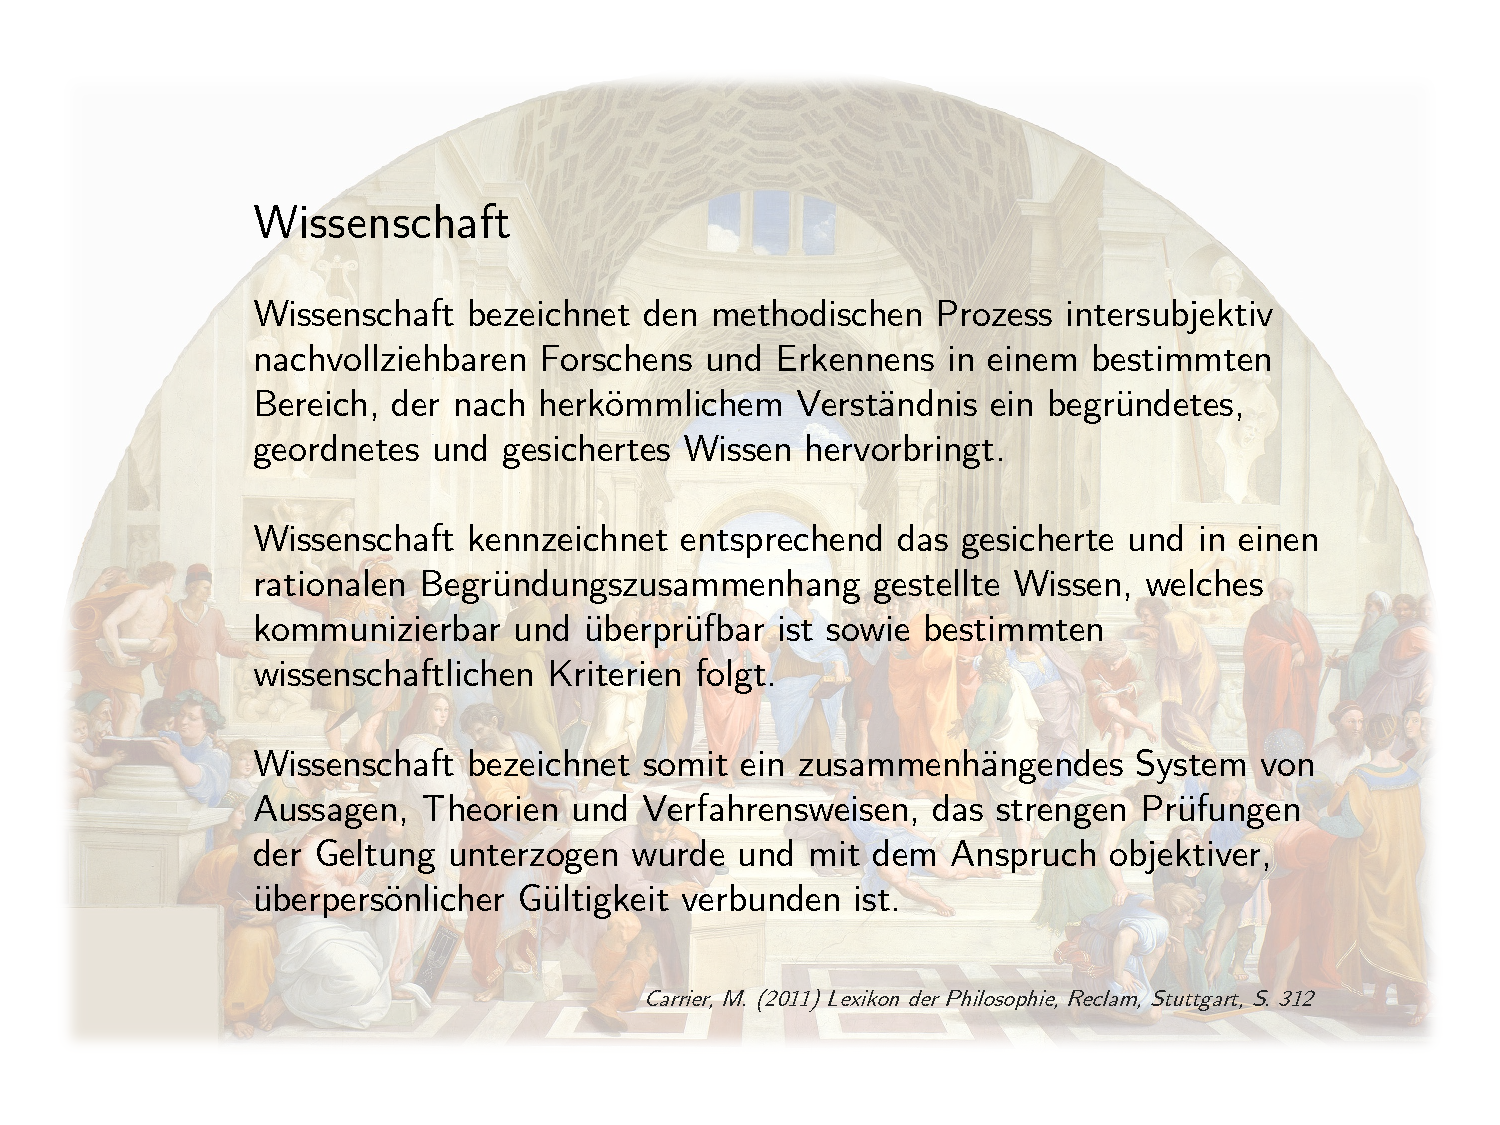
\includegraphics[width=1\linewidth]{1_Abbildungen/pfm_1_wissenschaft_definition} \end{center}
\end{frame}

\begin{frame}{Wissenschaft}
\protect\hypertarget{wissenschaft-1}{}
\setstretch{1.3}

\textcolor{darkblue}{Naturwissenschaften $\vert$ Science}

\begin{itemize}
\tightlist
\item
  Empirische Erforschung der Natur mit dem Ziel, Regelmäßigkeiten zu
  erkennen
\item
  Quantitatives Beobachten, messen, analysieren des Verhaltens der Natur
\item
  Grundlage zur Nutzbarmachung der Natur in den Ingeniuersdisziplinen
\item
  Physik, Chemie, Biologie, Medizin, \textcolor{darkblue}{Psychologie},
  Geologie, etc.
\end{itemize}

\textcolor{darkblue}{Geisteswissenschaften $\vert$ Humanities}

\begin{itemize}
\tightlist
\item
  Analytische Erforschung menschlicher Kultur
\item
  Qualitative Sinnsuche, informelle Kritik, Spekulation
\item
  Philosophie, Theologie, Geschichtswissenschaft, Literaturwissenschaft,
  etc.
\item
  Naturwissenschaftliche Theoriebildung
\end{itemize}

\textcolor{darkblue}{Formalwissenschaften $\vert$ Formal Sciences}

\begin{itemize}
\tightlist
\item
  Analyse formaler Systeme
\item
  Sprachwerkzeuge
\item
  Mathematik, Logik, theoretische Informatik, Rechtswissenschaft, etc.
\item
  Naturwissenschaftliche Theoriebildung
\end{itemize}
\end{frame}

\begin{frame}{Wissenschaft}
\protect\hypertarget{wissenschaft-2}{}
\setstretch{1.1}

\textcolor{darkblue}{Prinzipien der Erkenntnisgewinnung} \small

Prinzip der Intuition

\begin{itemize}
\tightlist
\item
  Unmittelbare Eingebung
\item
  Ökonomisch, aber risikobehaftet
\end{itemize}

Prinzip der Autorität

\begin{itemize}
\tightlist
\item
  Übernahme von Erkenntnissen von Autoritäten (Expert:innen)
\item
  Ökonomisch, aber risikobehaftet
\end{itemize}

Prinzip der Vernunft

\begin{itemize}
\tightlist
\item
  Erkenntnisgewinn in der Theorie nach formalen Regeln
\item
  Intersubjektiv, aber modellbasiert
\end{itemize}

Prinzip der Erfahrung

\begin{itemize}
\tightlist
\item
  Beobachtung und Experiment
\item
  Intersubjektiv, aber \emph{perse} unstrukturiert
\end{itemize}

\vspace{1mm}
\center

\textit{\textcolor{darkblue}{``Theorie ohne Erfahrung ist lediglich intellektuelles Spiel, Erfahrung ohne Theorie ist blind.''}}

\flushright{\textit{\textcolor{darkblue}{nach Immanuel Kant (vielleicht)}}}
\end{frame}

\begin{frame}{Wissenschaft}
\protect\hypertarget{wissenschaft-3}{}
\begin{center}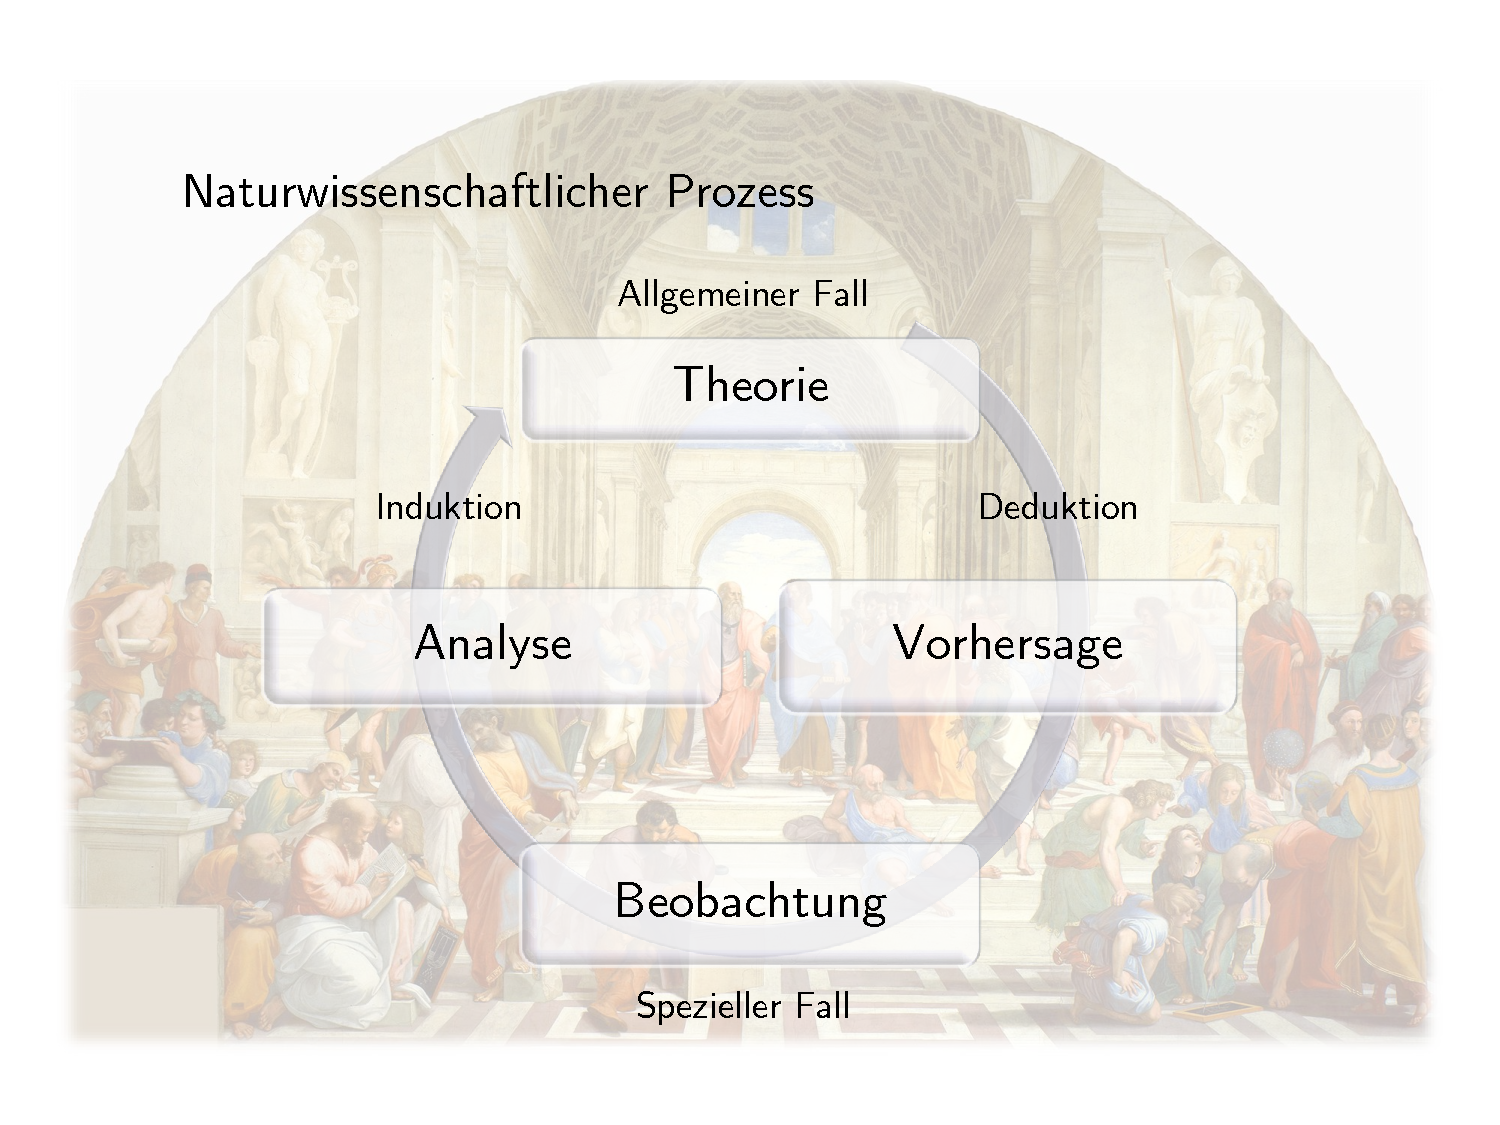
\includegraphics[width=0.95\linewidth]{1_Abbildungen/pfm_1_wissenschaft_prozess} \end{center}
\end{frame}

\begin{frame}{Wissenschaft}
\protect\hypertarget{wissenschaft-4}{}
\begin{center}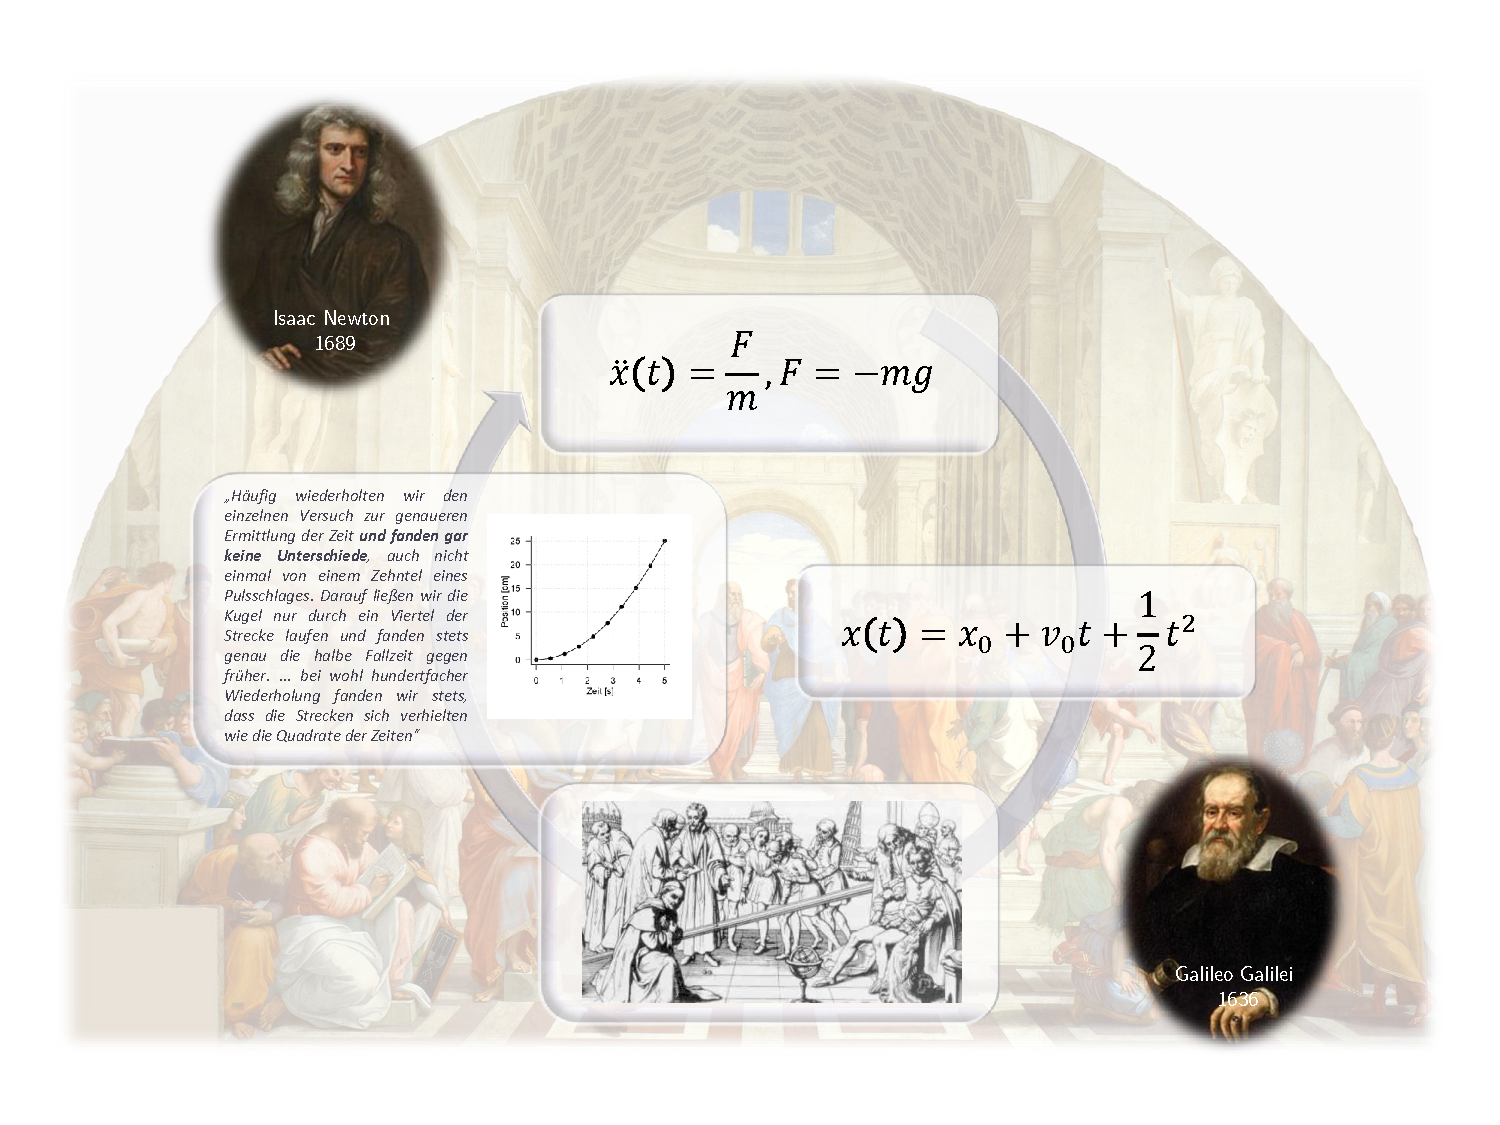
\includegraphics[width=0.95\linewidth]{1_Abbildungen/pfm_1_wissenschaft_prozess_freierfall} \end{center}
\end{frame}

\begin{frame}{Wissenschaft}
\protect\hypertarget{wissenschaft-5}{}
\begin{center}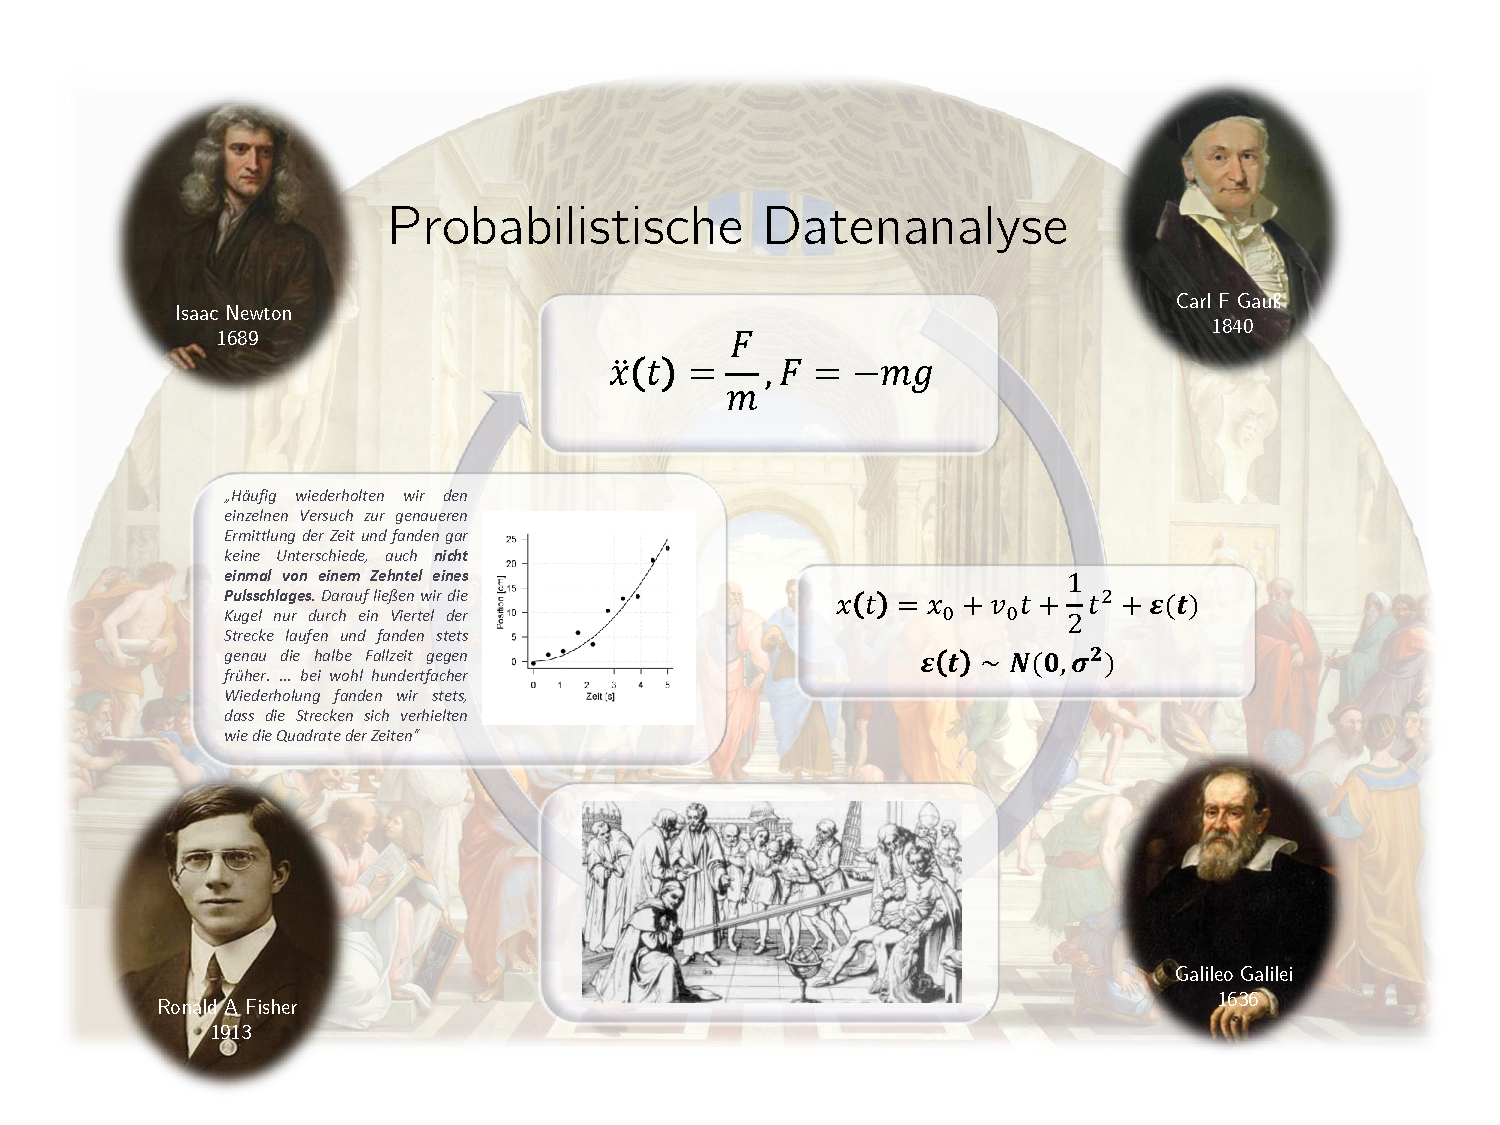
\includegraphics[width=0.95\linewidth]{1_Abbildungen/pfm_1_wissenschaft_prozess_freierfall_noise} \end{center}
\end{frame}

\begin{frame}{}
\protect\hypertarget{section-4}{}
\vfill
\setstretch{3}
\Large

Wissenschaft

\textbf{Theorien, Hypothesen, Experimente}

Variablen und Operationalisierung

Selbstkontrollfragen
\end{frame}

\begin{frame}{Theorien, Hypothesen, Experimente}
\protect\hypertarget{theorien-hypothesen-experimente}{}
\vspace{1mm}
\setstretch{1.2}

\textcolor{darkblue}{Theorien}

\small

``Eine Theorie ist ein Erklärungsmodell, das auf bestimmten Prinzipien
basiert. Eine Theorie stellt Einzelbeobachtungen in einen Zusammenhang.
Mithilfe einer Theorie können Verhaltensweisen oder Ereignisse in ein
System gebracht und Vorhersagen abgeleitet werden.''

\flushright

Myers (2010) \vspace{4mm}

\justifying

``Eine Theorie ist eine geordnete Menge von Konzepten oder Aussagen, die
ein Phänomen oder eine Gruppe von Phänomenen erklärt.''

\flushright

Gerrig et al. (2020) \vspace{4mm}

\justifying

``Eine Theorie ist ein System von Definitionen, Annahmen und
Schlussfolgerungen, welches einen Ordnungs- und Erklärungsversuch für
ein oder mehrere Phänomene darstellt.''

\flushright

Reiß and Sarris (2012)

\justifying

``Eine Theorie (ein Modell) ist ein System von intuitiv-verbal und
mathematisch formulierten Definitionen und Theoremen, die elementare
Grundannahmen zu Erklärung eines Phänomens der Wirklichkeit darstellen,
das die Herleitung quantitativer, informatisch-implementierbarer
Vorhersagen über beobachtbare Daten des Phänomens ermöglicht.''

\flushright

Ostwald (2021)
\end{frame}

\begin{frame}{Theorien, Hypothesen, Experimente}
\protect\hypertarget{theorien-hypothesen-experimente-1}{}
\textcolor{darkblue}{Theorien und Modelle} \small \setstretch{1.6}

Psycholog:innen unterscheiden manchmal zwischen den Begriffen
``Theorie'' und ``Modell''

\begin{itemize}
\tightlist
\item
  ``Nicht selten sind Modelle Bestandteile von Theorien''
\item
  ``Die allgemeinen theoretischen Prinzipien sind dann durch ein Modell
  repräsentiert''
\item
  ``Man unterscheidet Mathematische Modelle, Computermodelle, \ldots{}''
\end{itemize}

\flushright

(vgl. Reiß and Sarris (2012), S. 34 - 37)

\justifying

Psycholog:innen denken wohl, dass es Theorien auch ohne Modelle gibt
(oder so).

Psycholog:innen haben meist keine Erfahrung mit mathematischer oder
informatischer Modellbildung.

\(\Rightarrow\) Eine Unterscheidung zwischen Theorie und Modell ist
nicht zielführend.

\(\Rightarrow\) Mathematische und informatische Modellbildung ist für
naturwissenschaftliche Arbeit notwendig.

\large
\center

Modell = Theorie und Theorie = Modell
\end{frame}

\begin{frame}{Theorien, Hypothesen, Experimente}
\protect\hypertarget{theorien-hypothesen-experimente-2}{}
\textcolor{darkblue}{Hypothesen} \small

``Eine Hypothese ist eine überprüfbare Vorhersage, die aus einer Theorie
abgeleitet wird.''

\flushright

Myers (2010) \vspace{2mm}

\justifying

``Eine Hypothese ist eine vorläufige und prüfbare Erklärung der
Beziehung zwischen zwei oder meheren Ereignissen oder Variablen; oft als
Vorhersage formuliert, dass bestimmte Ereignisse aufgrund spezifischer
Bedingungen eintreten werden.

\flushright

Gerrig et al. (2020) \vspace{2mm}

\justifying

``Eine Hypothese ist eine experimentell zu prüfende Tatsachenbehauptung
bzw. präzise Angabe über die Art der erwarteten Abhängigkeitsbeziehung.
Sie enthält die exakte Festlegung der variierten Bedingungen und der
erwarteten Veränderungen, d.h. eine möglichst präzise Aussage
(Vorhersage) über die empirische Beziehung zwischen Ereignissen''

\flushright

Reiß and Sarris (2012)
\end{frame}

\begin{frame}{Theorien, Hypothesen, Experimente}
\protect\hypertarget{theorien-hypothesen-experimente-3}{}
\textcolor{darkblue}{Hypothese und Statistische Hypothese}

\small

Psycholog:innen verwechseln oft die Begriffe ``Hypothese'' und
``Statistische Hypothese''.

\(\quad\Rightarrow\) Der Begriff ``Hypothese'' und der Begriff der
``Statistischen Hypothese'' sind nicht gleich.

\begin{itemize}
\tightlist
\item
  \justifying ``Hypothese'' meint hier zunächst etwas wie ``aus der
  Theorie abgeleitete Datenvorhersage''.
\item
  Eine ``Statistische Hypothese'' (Nullhypothese, Alternativhypothese)
  ist eine Aussage über die Lage des wahren, aber unbekannten,
  Parameters im Parameterraum eines statistischen Modells.
\end{itemize}

Hypothesen können manchmal als Statistische Hypothesen formuliert
werden.

\(\quad\Rightarrow\) Hypothesen müssen nicht als Statistische Hypothesen
formuliert werden.

\(\quad\Rightarrow\) Es gibt mehr datenanalytische Verfahren als
Frequentistisches Hypothesentesten.

Die Annahme oder Ablehnung von Statistischen Hypothesen sind
Quantifizierungen von Unsicherheit, keine abschließenden binären
Urteile. Keine Hypothese wird sich jemals als absolut ``falsch'' oder
absolut ``richtig'' erweisen.
\end{frame}

\begin{frame}{Theorien, Hypothesen, Experimente}
\protect\hypertarget{theorien-hypothesen-experimente-4}{}
\textcolor{darkblue}{Probabilistische Datenvorhersage statt Hypothese}
\small \setstretch{1.3}

Der von Psycholog:innen propagierte Hypothesenfetisch ist problematisch:

\begin{itemize}
\item Verwechselung von Hypothesen und Statistischen Hypothesen
\item Abwertung wichtiger naturwissenschaftlicher Beiträge wie zum Beispiel
\begin{itemize}
\begin{small}
\item[$\circ$] (Mathematische) Modellentwicklung und (analytische/simulierende) Modellvalidation
\item[$\circ$] Datenerhebung, Datenaufbereitung, Datenbereitstellung
\item[$\circ$] Exploratorisch-charakterisierende Forschungsprojekte
\end{small}
\end{itemize}
\end{itemize}

Der Hypothesenfetisch hat die Qualität (psychologischer) Forschung
gemindert:

\begin{itemize}
\tightlist
\item
  p-Hacking: Datenselektion bis zum Ablehnen der (statistischen)
  Nullhypothese
\item
  HARKING: Hypothesizing After Results are Known (Pseudohypothesen)
\end{itemize}

Entscheidend für das naturwissenschafltiche Paradigma ist es, dass aus
Theorien quantitative Vorhersagen beobachtbarer Daten abgeleitet werden,
deren explanatorische Unsicherheit probabilistisch quantifiziert werden
kann und die Theorievergleiche ermöglicht.

\(\Rightarrow\) An die Stelle des ``Hypothesentestens'' sollte das
``Theorievergleichen'' treten.
\end{frame}

\begin{frame}{Theorien, Hypothesen, Experimente}
\protect\hypertarget{theorien-hypothesen-experimente-5}{}
\textcolor{darkblue}{Experimente} \small

``Ein Experiment ist eine Untersuchung, bei welcher
Untersuchungsleitende aktiv und gezielt eine Intervention durchführen,
um die Effekte der Intervention zu beobachten''

\flushright

Shadish, Cook, and Campbell (2001) \vspace{2mm}

\justifying

``Ein Experiment ist eine empirische Untersuchung, bei der gezielt
bestimmte Bedingungen (Stufen der \emph{unabhängigen Variable})
hergestellt werden und in ihren Auswirkungen auf ausgewählte
\emph{abhängige Variablen} beobachtet werden''.

\flushright

Bortz and Döring (2006) \vspace{2mm}

\justifying

``Ein Experiment ist ein systematischer Beobachtungsvorgang, aufgrund
dessen der Versuchsleiter (sic) das jeweils interessierende Phänomen
planmäßig erzeugt und variiert sowie gleichzeitig systematische und/oder
unsystematische Störfaktoren durch hierfür geeignete Techniken
kontrolliert''

\flushright

Reiß and Sarris (2012)
\end{frame}

\begin{frame}{Theorien, Hypothesen, Experimente}
\protect\hypertarget{theorien-hypothesen-experimente-6}{}
\textcolor{darkblue}{Experimente} \vspace{5mm} \setstretch{1.7}

\begin{minipage}{.3\linewidth}
\begin{center}
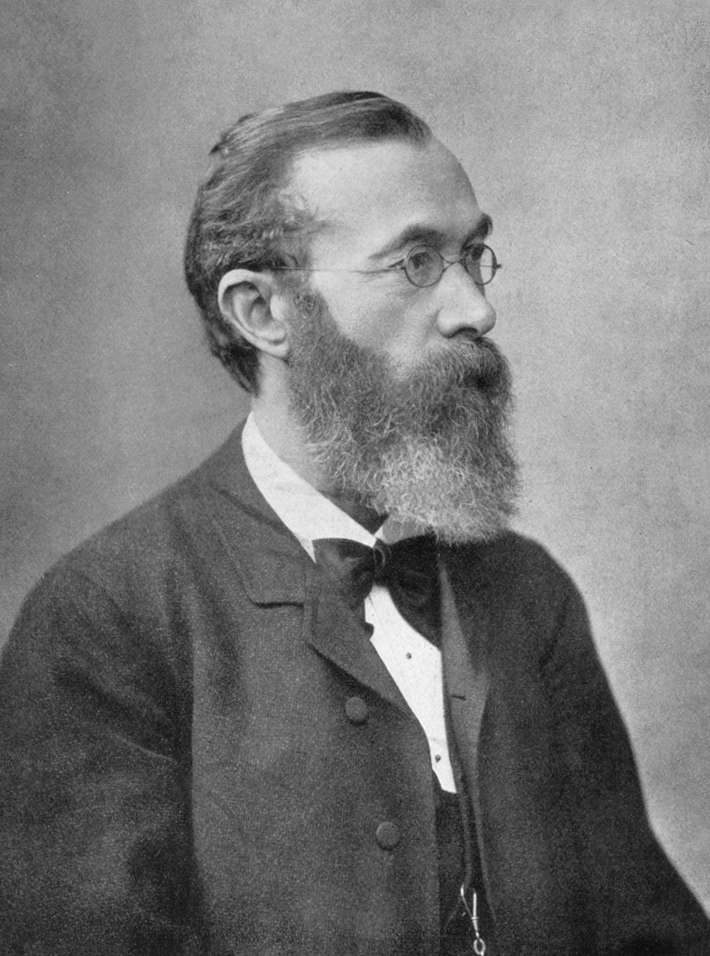
\includegraphics[scale=1]{1_Abbildungen/pfm_1_wundt.jpg}

\footnotesize
Willhelm Wundt (1832 - 1920)

\end{center}
\end{minipage}
\hspace{7mm}
\begin{minipage}{.7\linewidth}
\vspace{-5mm}
\begin{large}
Experimentkriterien nach Wundt
\vspace{1mm}
\begin{itemize}
\itemsep2mm
\item Willkürlichkeit
\item Variierbarkeit
\item Wiederholbarkeit
\end{itemize}
\end{large}
\end{minipage}
\vspace{.7cm}
\end{frame}

\begin{frame}{Theorien, Hypothesen, Experimente}
\protect\hypertarget{theorien-hypothesen-experimente-7}{}
\textcolor{darkblue}{Experimente vs. Quasiexperimente vs. Korrelationsstudien}

Experiment

\begin{itemize}
\tightlist
\item
  Randomisierte kontrollierte Studie
\item
  Die Untersuchungseinheiten werden den Versuchsbedingungen zufällig
  zugeordnet
\item
  Beispiel: Online Psychotherapie vs.~Klassische Psychotherapie bei
  Depression
\end{itemize}

\normalsize

Quasiexperiment

\begin{itemize}
\tightlist
\item
  Nicht-randomisierte kontrollierte Studie
\item
  Untersuchung natürlich bzw. bereits bestehender Gruppen
\item
  Beispiel: Online Psychotherapie bei Depression vs.~Schizophrenie
\end{itemize}

\normalsize

Korrelationsstudie

\begin{itemize}
\tightlist
\item
  Nicht-randomisierte, nicht kontrollierte Studie
\item
  Beobachtungsstudie ohne Intervention
\item
  Beispiel: Analyse von Paneldaten
\end{itemize}
\end{frame}

\begin{frame}{Theorien, Hypothesen, Experimente}
\protect\hypertarget{theorien-hypothesen-experimente-8}{}
\textcolor{darkblue}{Datenerhebung statt Experiment} \small
\setstretch{1.3}

Der von (Experimental)Psycholog:innen propagierte Experimentenfetisch
ist problematisch:

\begin{itemize}
\tightlist
\item
  Abwertung anderer wichtiger naturwissenschaftlicher Beiträge
\item
  Fokus auf experimentelles Design anstatt integrierter Betrachtung von
  Design und Analyse
\item
  Es gibt keinen prinzipiellen Unterschied zwischen ``Hypothesentests''
  und ``Korrelation''
\item
  Experimentaldatenbesitzgier verhindert wissenschaftlichen Fortschritt
\end{itemize}

\vspace{1mm}

Datenerhebungen finden (mindestens) in einem zweidimensionalen
Erhebungsraum statt

\center

Holistisch

\(\Uparrow\)

\(\,\,\,\) Kontrolliert \(\Leftarrow \quad \Rightarrow\) Unkontrolliert

\(\Downarrow\)

Reduktionistisch

Entscheidend ist die kritische Evaluation der Lage einer Datenerhebung
in diesem Kontinuum

\center

Niemand sagt mehr ``Experiment'', jeder sagt ``Studie'' heutzutage.
\end{frame}

\begin{frame}{}
\protect\hypertarget{section-5}{}
\vfill
\setstretch{3}
\Large

Wissenschaft

Theorien, Hypothesen, Experimente

\textbf{Variablen und Operationalisierung}

Selbstkontrollfragen
\end{frame}

\begin{frame}{Variablen und Operationalisierung}
\protect\hypertarget{variablen-und-operationalisierung}{}
\textcolor{darkblue}{Variable}

Eine Variable ist etwas, das durch Veränderlichkeit charakterisiert ist.
\vspace{5mm}

\textcolor{darkblue}{Konstrukt}

Ein Konstrukt ist ein in der Theorie generierter Erklärungsbegriff, der
sich nur indirekt und unter Zuhilfenahme operationaler Definitionen
empirisch erfassen lässt. \vspace{5mm}

\textcolor{darkblue}{Operationalisieren}

Operationalisieren bezeichnet den Prozess der Umsetzung eines Konstrukts
in eine empirisch messbare Variable.

\vspace{5mm}
\footnotesize
\flushright

Reiß and Sarris (2012)
\end{frame}

\begin{frame}{Variablen und Operationalisierung}
\protect\hypertarget{variablen-und-operationalisierung-1}{}
\textcolor{darkblue}{Unabhängige Variable (UV)}

Etwas, das in einer Studie systematisch variiert wird, um seine
Auswirkung auf eine oder mehrere abhängige Variable(n) zu untersuchen.
\vspace{3mm}

\textcolor{darkblue}{Abhängige Variable (AV)}

Etwas, das in einer Studie erfasst wird, um zu überprüfen, wie sich
systematisch variierte unabhängige Variablen auswirken \vspace{3mm}

\textcolor{darkblue}{Beispiele}

\small

\begin{itemize}
\tightlist
\item
  Einfluss von Alkoholkonsum (UV) auf Reaktionszeiten (AV)
\item
  Einfluss des Erziehungstils (UV) auf die Kreativität von Kindern (AV)
\item
  Einfluss der Belohnungsanzahl (UV) auf die Leistungsmotivation (AV)
\item
  Einfluss des Entscheidungskontext (UV) auf das Entscheidungsverhalten
  (AV)
\end{itemize}
\end{frame}

\begin{frame}{Variablen und Operationalisierung}
\protect\hypertarget{variablen-und-operationalisierung-2}{}
\textcolor{darkblue}{Diskrete Variablen}

Diskrete (kategoriale) Variablen sind Variablen, die nur eine endliche
Anzahl an verschiedenen Werten annehmen und meist durch ganze Zahlen
repräsentiert sind. \vspace{4mm}

\textcolor{darkblue}{Kontinuierliche Variablen}

Kontinuierliche Variablen sind Variablen, die unendlich viele Werte
annehmen können und meist durch die reellen Zahlen repräsentiert sind.
\vspace{4mm}

\textcolor{darkblue}{Einordnung einer Variable als diskret oder kontinuierlich ist eine Modellierungsannahme}

\center
\begin{tabular}{ll}
Geschlecht        & m/w vs. m/w/d vs. Kontinuum                        \\
Alter             & Zeit als reelle Zahl vs. 20, 21, 22, ..., 100      \\
Reaktionszeiten   & Zeit als reelle Zahl vs. floating point numbers
\end{tabular}
\end{frame}

\begin{frame}{Variablen und Operationalisierung}
\protect\hypertarget{variablen-und-operationalisierung-3}{}
\setstretch{2.2}

\textcolor{darkblue}{Anmerkungen}

Die Begriffsdefinitionen UV und AV sind kontraintuitiv.

Variablentypen sollten nicht mit mathematischen Variablen verwechselt
werden.

Alle Variablentypen können als Zufallsvariablen modelliert werden oder
auch nicht.

Die Zuteilung messbarer Entitäten zu Variablentypen ist ein
subjektiv-kreativer Prozess:

\center

``One researcher's signal is another researcher's noise.''
\end{frame}

\begin{frame}{}
\protect\hypertarget{section-6}{}
\vfill
\setstretch{3}
\Large

Wissenschaft

Theorien, Hypothesen, Experimente

Variablen und Operationalisierung

\textbf{Selbstkontrollfragen}
\end{frame}

\begin{frame}{Selbstkontrollfragen}
\protect\hypertarget{selbstkontrollfragen}{}
\footnotesize
\setstretch{2}

\begin{enumerate}
\tightlist
\item
  Diskutieren Sie die Begriffe Naturwissenschaft, Geisteswissenschaft
  und Formalwissenschaft.
\item
  Beschreiben Sie den naturwissenschaftlichen Prozess.
\item
  Geben Sie die Definition einer Theorie nach Reiß and Sarris (2012)
  wieder.
\item
  Geben Sie die Definition einer Theorie nach Ostwald (2021) wieder.
\item
  Geben Sie die Definition einer Hypothese nach Reiß and Sarris (2012)
  wieder.
\item
  Geben Sie die Definition eines Experimentes nach Reiß and Sarris
  (2012) wieder.
\item
  Nennen und erläutern Sie die Experimentkriterien nach Wundt.
\item
  Erläutern Sie die Begriffe Experiment, Quasiexperiment und
  Korrelationsstudie.
\item
  Definieren Sie die Begriffe Variable, Konstrukt, und
  Operationalisierung nach Reiß and Sarris (2012).
\item
  Definieren Sie die Begriffe Unabhängige Variable und Abhängige
  Variable.
\item
  Definieren Sie die Begriffe Diskrete Variable und Kontinuierliche
  Variable.
\end{enumerate}
\end{frame}

\begin{frame}{References}
\protect\hypertarget{references}{}
\footnotesize

\hypertarget{refs}{}
\begin{CSLReferences}{1}{0}
\leavevmode\vadjust pre{\hypertarget{ref-bortz_2006}{}}%
Bortz, Jürgen, and Nicola Döring. 2006. \emph{{Forschungsmethoden und
Evaluation: für Human- und Sozialwissenschaftler}}. 4., überarb. Aufl.,
{[}Nachdr.{]}. {Springer-Lehrbuch Bachelor, Master}. {Heidelberg}:
{Springer-Medizin-Verl}.

\leavevmode\vadjust pre{\hypertarget{ref-gerrig_2020}{}}%
Gerrig, Richard J., Philip G. Zimbardo, Ralf Graf, and Richard J.
Gerrig. 2020. \emph{{Psychologie}}. 18., aktualis. Aufl., {[}Nachdr.{]}.
{ps psychologie}. {München}: {Pearson Studium}.

\leavevmode\vadjust pre{\hypertarget{ref-myers_2010}{}}%
Myers, David G. 2010. \emph{Psychology}. 9th ed. {New York}: {Worth
Publishers}.

\leavevmode\vadjust pre{\hypertarget{ref-reiss_2012}{}}%
Reiß, Siegbert, and Viktor Sarris. 2012. \emph{{Experimentelle
Psychologie: von der Theorie zur Praxis}}. {Pearson Studium
Psychologie}. {München}: {Pearson}.

\leavevmode\vadjust pre{\hypertarget{ref-shadish_2001}{}}%
Shadish, William R., Thomas D. Cook, and Donald T. Campbell. 2001.
\emph{Experimental and Quasi-Experimental Designs for Generalized Causal
Inference}. {Boston}: {Houghton Mifflin}.

\end{CSLReferences}
\end{frame}

\end{document}
